\documentclass{ltjsbook}
\usepackage{docmute} 
\usepackage{../../myStyle} 


\begin{document}
\chapter{Points to note in null hypothesis testing}
\label{m19_NHST2}
Last time, we discussed hypothesis testing for the null hypothesis. How did you find the explanation?
First, we establish a null hypothesis, such as "there is no relationship" or "there is no difference," and set the alternative hypothesis as what we actually want to claim. Then, by using the logic of proof by contradiction, we conclude by rejecting the null hypothesis with evidence that would rarely occur under the null hypothesis, thereby accepting the alternative hypothesis. It is important to note that this approach involves somewhat unconventional thinking. Have you also understood that we reject the null hypothesis based on the fact that the data we have obtained would seldom occur under the null hypothesis?

In this explanation, we will discuss how to report and interpret the results of the null hypothesis test. It is important to note that there are many misconceptions and misuses of the test, as it is a widely used but somewhat unnatural method that relies on counterintuitive reasoning and probabilities. In fact, the author believes that the test may not be suitable for beginners, who may struggle with understanding the underlying concepts. Even in past research papers, some mistakes in the application and interpretation of the test may be present, even in articles written and reviewed by professional researchers such as university professors. This may be due to various reasons, including the fact that in the past when computers were not as developed, researchers had to resort to alternative methods that were not necessarily correct. It is important to always strive to use the most appropriate and accurate methods in research, and to avoid practicing incorrect methods knowingly. Therefore, it is recommended to gain a solid foundational knowledge and to avoid jumping to easy but incorrect conclusions.

In the following section, we will briefly explain how to report the results of a null hypothesis test.

\section{Reporting Results}
The hypothesis testing involves a model contest between the null hypothesis and alternative hypothesis, therefore the result needs to clearly indicate the winner. It should be specified whether the null hypothesis has won or the alternative hypothesis. By the way, accepting the hypothesis winning is called "acceptance", whereas rejecting it is called "rejection". Therefore, it will be either "rejecting the null hypothesis and accepting the alternative hypothesis" or "accepting the null hypothesis and rejecting the alternative hypothesis" depending on whether the null hypothesis has been rejected and the alternative hypothesis has been accepted, or the null hypothesis has been accepted and the alternative hypothesis has been rejected.

Also, it is necessary to report the value that was used for the hypothesis test - the test statistic - along with the results. For example, in the case of testing a correlation coefficient, the $t$-statistic is commonly used and reported. Since the $t$-statistic follows a $t$-distribution and is adjusted by degrees of freedom that depend on the sample size, it is also necessary to report the degrees of freedom. In the previous example, the correlation coefficient of $r = 0.50$ was obtained from a dataset with a sample size of 20, and it was concluded that the result is statistically significant. To report this result, it should be presented as follows:
\begin{quote}
    A hypothesis test was conducted for a sample correlation coefficient of $r=0.50$ obtained from a sample, which was statistically significant with $t(18)=2.450, p=0.0248$.
\end{quote}

As a point of writing, it is important to include the statistical values and to note that they should be in italics\footnote{It is common practice in psychology and other academic writing to format statistical values and titles of books in italics. This is specified in the Publication Manual of the American Psychological Association and is generally followed by publishing standards set by psychological associations in Japan.}. Additionally, it is necessary to include the probability value ($p$-value) associated with the observed statistical value.

The basic method of presenting the probability in $p$-values is by depicting the probability itself, as shown in the above example. However, in the past, criteria for judgments such as $p<0.05$ or $p<0.01$ were used. This was a remnant from the days of manual testing, when there were no statistical environments like R, and direct calculations of probability were impossible. In those days, the only option was to use numerical tables containing representative probability distributions\footnote{In the past, there were books containing a list of numerical probability distributions. Also, some probability textbooks include a part of the table in their appendices.}, and it was impossible to calculate values precisely to decimal places\footnote{For example, t-distributions vary according to degrees of freedom, but if they were written down one by one for degrees of freedom $1,2,3,\cdots$, the appendix would require many pages no matter how it was organized. So, only a rough range was listed for the latter half of the degrees of freedom, such as "$1,2,3,\cdots 10,15,30,50$." You may wonder at a time like this, "What should I do if the degrees of freedom are 18?" In such a case, you had to take the value of 15 degrees of freedom closest to your data, which was more stringent, as the substitute. Therefore, specific p-values could not be written down.} Nowadays, there is no such problem, so let's write down $p$-values directly.

\section{What Does "Statistically Significant" Mean?}
\label{statistical_significant}
So far, we have conducted testing of the mean value and correlation coefficient (of one variable).
The case discussed pertained to situations when the observed values significantly deviate from the expected means or when there is/isn't a correlation in the population, but ultimately the decision comes down to rejecting/accepting the null hypothesis.

At that time, when the null hypothesis was rejected, it was referred to as "statistically significant." This signifies that there is statistical meaning. However, it is important to note what it means to be statistically significant.
Let's recall what happened during the correlation coefficient test. The null hypothesis was that $\rho=0$. Since this was rejected, the conclusion was that there is a statistically significant correlation coefficient. However, it would be more accurate to say that "we cannot conclude that the population correlation is 0". The part where we go from "cannot say it's unrelated" to "it's related" involves a slight leap\footnote{It's like when someone tells you "I don't dislike you", but it doesn't necessarily mean they like you either.}.

The person who came up with this null hypothesis testing is R.A. Fisher, and he intended to use it as a check for experimental procedures by saying that if the null hypothesis is rejected, "something strange is happening in reality, so the experimental procedure should be reviewed." E. Pearson and J. Neyman applied this method to the criterion of judging that "rejecting the null hypothesis = adopting the alternative hypothesis." Psychology has used null hypothesis testing in this way as a result of this trend. In that sense, it is being used in a more practical (in other words, responsible for practical use) way than the original founder intended.

As mentioned before, it's important to note that the expression used in the table obscures information about the size of the actual correlation coefficient and the difference in means. While the final decision relies solely on the $p$-value, looking at this number alone doesn't provide any insight into how large the correlation coefficient was or how much the means differed. Even if we examine the result that says, "it was statistically significant, there was a relationship," we could end up with an odd conclusion if the sample correlation coefficient was actually only $r=0.1$\footnote{In fact, once a sample size surpasses 271 people, a sample correlation coefficient of 0.1 becomes statistically significant at the 5\% level.}. Therefore, if we declare that "it's statistically significant! It can't be uncorrelated!" based solely on the fact that the sample correlation coefficient was 0.1, we're likely to come to a strange conclusion when we discuss the results that there was a relationship.

However, in reality, we often get caught up in these surface-level uses. Especially when conducting research, there is a feeling of not wanting to admit that our efforts were in vain. Therefore, we may force ourselves to examine the relationship between two variables, even if there is no clear significance, thinking that it must mean something because it was found to be statistically significant. This will invalidate all the effort we put into collecting the data in the first place.

As the sample size increases, the p-value generally decreases, making it easier to reject the null hypothesis. Figure \ref{fig::18_02} plots the sample size on the horizontal axis and the p-value on the vertical axis for sample correlation coefficients of $r=0.5,0.3,0.1$. The significance level of 5% is shown as a dotted line, but as the sample size increases, the p-value decreases.

\begin{figure}[ht]
    \centering
    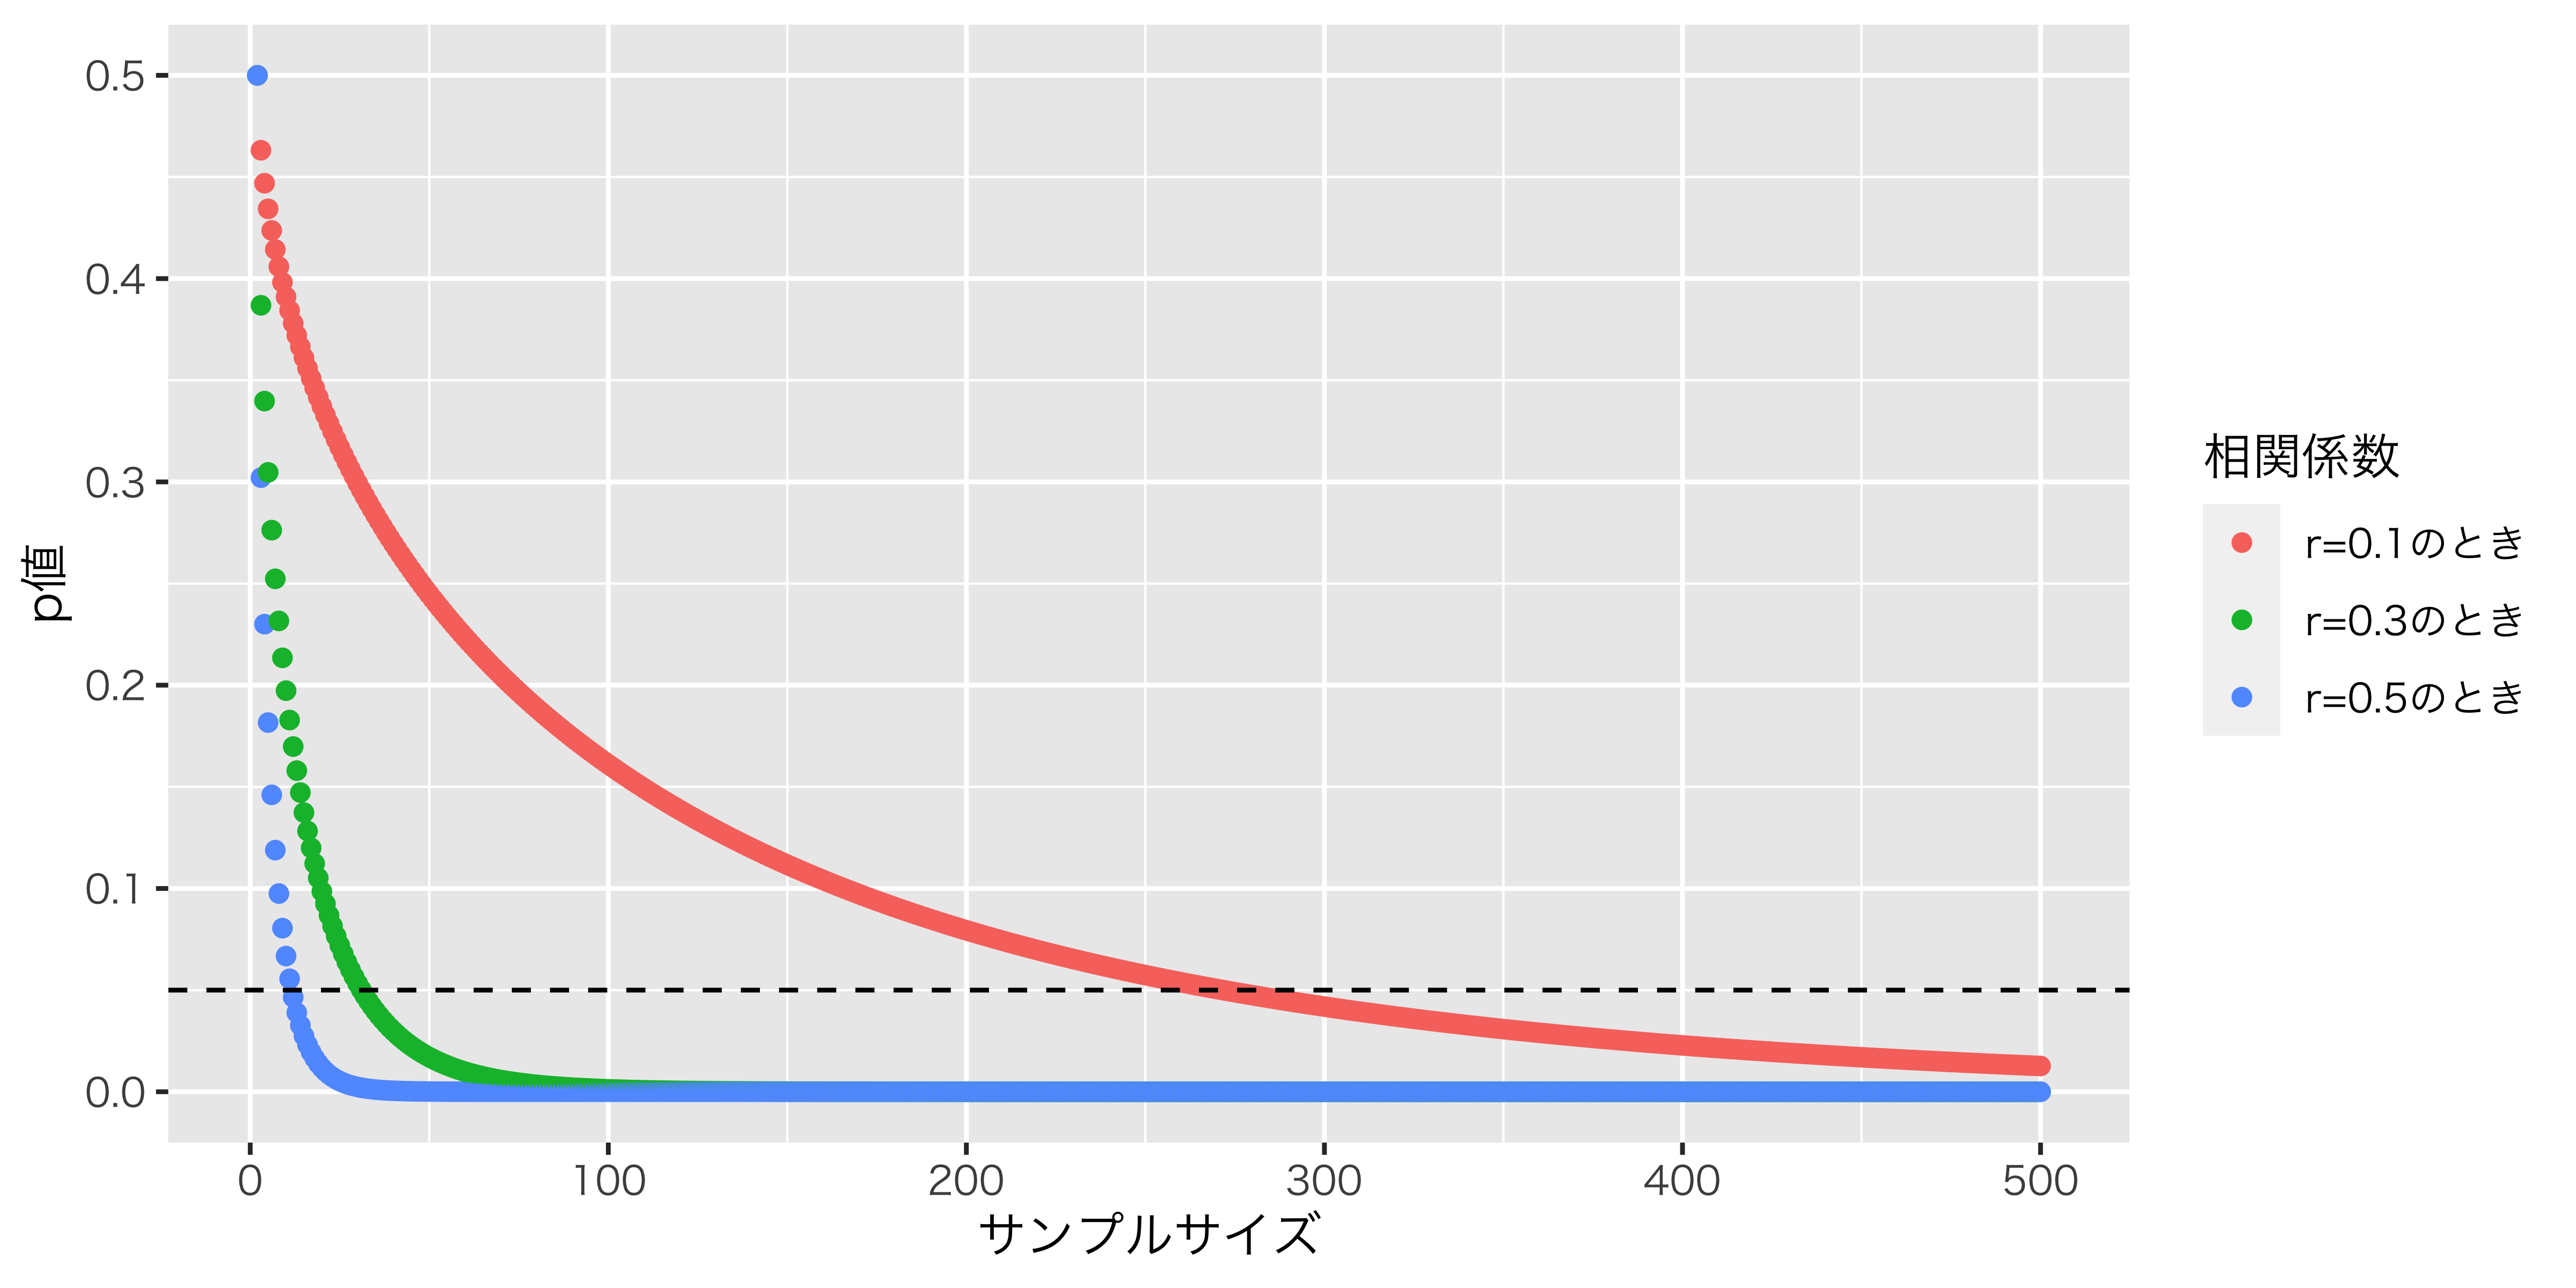
\includegraphics[keepaspectratio,width=0.8\linewidth]{../images/18_NHST/Rplot18_02.png}
    \caption{Relationship between Sample Size and $p$-value}
    \label{fig::18_02}
\end{figure}


Regardless of where it starts, this descent pattern takes the same form, so the test will eventually become significant as the sample size increases. This has created a strange trend in research practice where there is a belief that \underline{if you want to make it significant}, simply take a larger sample size, meaning the harder you work, the better.

However, don't you think that depending on "effort" that "will become significant if you try hard" in scenes where scientific accuracy is important is absurd? The logic of "worked hard" $\to$ "became significant" $\to$ "the author's claim is correct" is not valid. Changing the results to suit one's own convenience is not the right kind of effort.

The null hypothesis test is an excellent technique for "judging" the population from a sample. However, it is important to be careful with the expressions used and their interpretations. Otherwise, it may lead science in the wrong direction. Unfortunately, there have been cases in the history of psychology of such misunderstandings, which are called "Questionable Research Practices" or QRPs for short. Some examples of this include increasing the sample size "to obtain significant results" or repeating tests "until significant results are obtained." These practices are still happening in some research environments. However, if these practices occur, scientific debates will be based on "erroneous results (interpretations)," and subsequent studies may collapse, wasting years of effort. While data falsification and plagiarism are clearly malicious acts, "working hard to increase data" may seem like a sincere and honest research attitude, so it is a tricky problem that can mislead people. Effort can mislead people. Please proceed with your research with care, so that you are not deceived or led down the wrong path.

\section{Two types of errors in hypothesis testing}
\subsection{What is a $p$-value?}
\label{TypeI_II_Error}
By the way, hypothesis testing of the null hypothesis is a "judgment" application of "estimation." This judgment is made probabilistically, but humans are not particularly skilled in probabilistic thinking, so it is not uncommon to accidentally misunderstand. Let's think about when correct or incorrect judgments occur.

I have been using a number called the p-value to explain it since earlier, but what exactly does this p-value represent? Let's consider the following options.

\begin{itemize}
    \item Probability that the null hypothesis is true
    \item Number indicating the validity of the null hypothesis
    \item Number indicating the strength of significance level (the smaller the $p$-value is, the stronger the effect is)
    \item Number indicating the strength of the test
\end{itemize}


Actually, the correct answer is none of the above. Sorry for the sneaky options.

The two options above, "the probability of generating a null hypothesis" and "the number representing the correctness of a null hypothesis," are common misunderstandings.
Hypothesis testing begins with the assumption of a null hypothesis. As we mentioned in the case of correlation testing, we pick up a sample from a world where the population correlation is 0. Since we assume a world with a certain population correlation, the probability of the null hypothesis arising is 100\%, and the correctness of the null hypothesis is also 100\%, because we assumed it!

This is not a number that represents the degree of significance. Certainly, if there is a large difference or if it is far from the world of the null hypothesis, the realized value of the test statistic will be larger and the $p$-value will be smaller. However, what the $p$-value indicates is only the \underline{probability of observing the test statistic\underline{(s) under the null hypothesis}}. It is a number that represents the hypothetical space of the null hypothesis and does not indicate anything about the actual statistics.

It is not a measure of the strength of a hypothesis test. While a smaller p-value indicates a higher level of rarity, it only reflects the rarity within the hypothetical space of the null hypothesis and does not provide information on how much the null hypothesis has been defeated by the alternative hypothesis. Therefore, thinking that a smaller p-value is more impressive can lead to a misunderstanding of the essence of the hypothesis test.

How should we think about the correctness or incorrectness of testing? In fact, this too has the difficulty of probabilistic expressions.
In the final step of the hypothesis testing, there was a process of "determining whether the initial hypothesis is correct or incorrect." However, there are two ways in which this judgement can be incorrect. That is, there are errors in "rejecting the null hypothesis when it is actually true" and "accepting the null hypothesis when it is actually false."

\begin{figure}[ht]
    \centering
    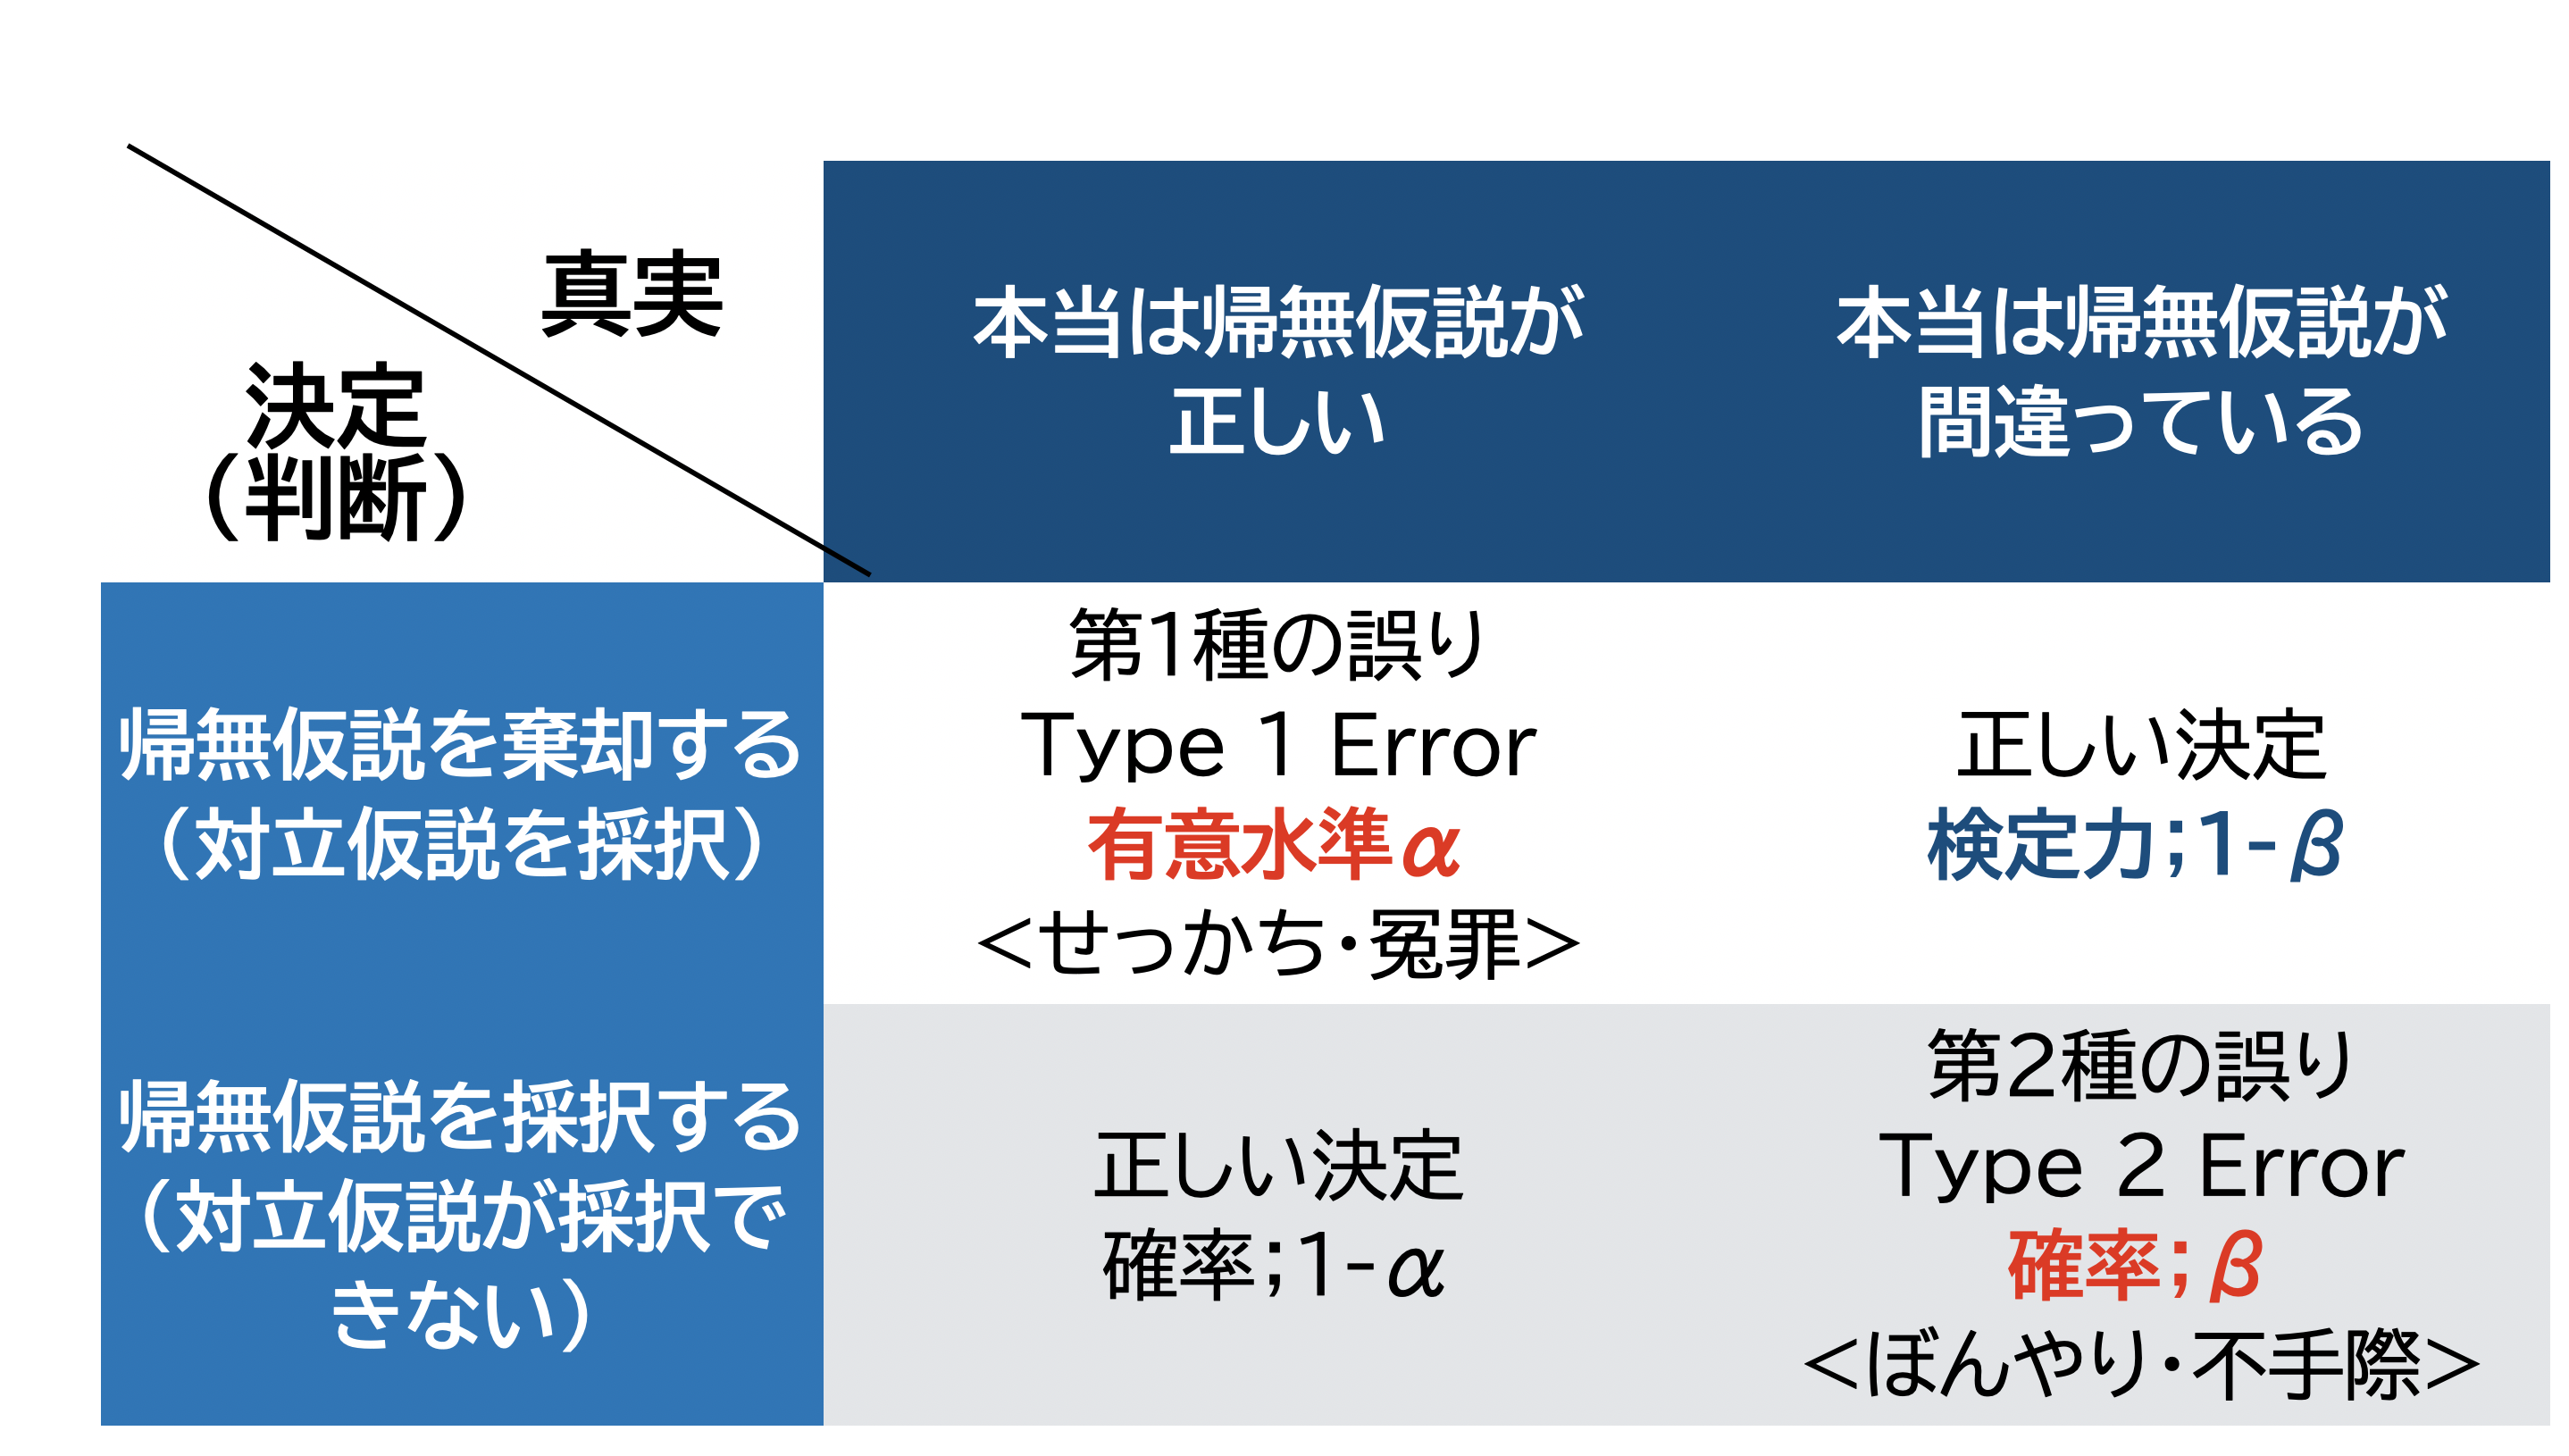
\includegraphics[keepaspectratio,width=0.8\linewidth]{../images/18_NHST/slide18_01.png}
    \caption{Two types of mistakes}
    \label{fig::18_03}
\end{figure}

I have written the combinations of incorrect ways in Figure \ref{fig::18_03}. Accepting the null hypothesis when it is true is a correct decision, as well as rejecting it when it is false. However, it is a mistake to reject the null hypothesis when it is true, and to accept it when it is false.

The null hypothesis is a conclusion that there is no difference or effect, often referred to as a "null" conclusion. Imagine a scenario where we are considering whether a newly developed drug has a therapeutic effect. The null hypothesis in this case would be that the drug has no effect. Rejecting the null hypothesis when there is no significant effect is dangerous, as it can lead to incorrect conclusions and negative effects on patients (such as side effects). This type of error, where we reject the null hypothesis when we shouldn't, is called a Type I Error, with a probability denoted as $\alpha$. Traditionally, the significance level is set at 5%, meaning that $\alpha=0.05$. However, this level can be freely determined, ranging from 1% to 10%, with consideration given to the importance of making this type of mistake.

On the other hand, it is a disappointing case when we accept the null hypothesis despite there being an effect (i.e., when the null hypothesis is incorrect), as we fail to identify the effect we were looking for. However, at least in this case, there are no practical problems that could harm patients. This case is called a Type II Error, with probability typically denoted as $\beta$. However, due to the nature of this error, where we cannot estimate how non-null the state is, we cannot estimate the size of $\beta$. We can only hope to identify the effect if it exists. In the table in Figure \ref{fig::18_03}, the rows indicate different worlds, and the probability of rejecting the null hypothesis in the "incorrect null hypothesis world" in the right-most column is denoted as $\beta$, while the probability of properly identifying an effect is $1-\beta$, called the statistical power. Checking if our analysis has enough power is important for the proper procedure of research.

\subsection{Inflation of $\alpha$}
\label{alphaInfration}
Earlier, we discussed how setting a significance level of 5% is equivalent to setting $\alpha$. Essentially, the idea is to design criteria for judgment to prevent careless mistakes of claiming there is an effect when there isn't one.
Without changing the TeX code, please translate the following Japanese text into English:

Keeping that in mind, consider the following analogy\footnote{This analogy is taken from \citet{BA33892274}.}.
\begin{quote}
    In the basement of a certain restaurant, many wines are stored, but one out of every 20 bottles is a defective product that has become sour. When a customer comes in and orders one bottle of wine, the sommelier will sweat cold 20 times out of 1.
    At the parties held at this restaurant, wine is served in units of 10 bottles, but if even one sour wine is included, the party will be ruined. How much does the sommelier have to apologize during the party?
\end{quote}


It seems like a shady restaurant with a questionable sommelier. While I wouldn't want to visit such a place in reality, of course, this is just a fictional story. The statement that there is one bad wine among every 20 is a metaphor for the 5% significance level in hypothesis testing.
So, in other words, there is a risk of a 5% error rate in judgement.
Setting the standard for careless mistakes at 5\% means that, in other words, there is a high probability of 95\% that the judgment is correct, so it can be said that there are usually no problems. That means there is only one mistake every 20 times at this restaurant.

However, when the party started, a bunch of wine was offered all at once. In one party, there were 10 bottles of wine available.
Let's say you have brought two bottles of wine. The risk rate is 5\%, and the safety rate is 95\%, but this applies to each individual bottle. The probability of both bottles being safe in succession is $0.95\times 0.95=0.9025$. In other words, the probability of at least one of the bottles being unsafe is $1-0.9025=0.0975$, which is almost 10\%.

Similarly, if you bring 10 together, the probability of at least one of them being incorrect is $1-(0.95)^{10}=0.4013$, which is 40%.
In other words, if you bring 10 of them together, you can see that the risk rate of 5% when taking one at a time jumps up to 40%.

Let's return to the world of psychology. In psychology, when verifying experimental results, it is judged with a significance level of 5%.
Now, let's say there is a diligent researcher who is studying a phenomenon from various angles and conducting numerous statistical tests to come to a conclusion. This researcher is very careful and thorough, so they consider 10 experiments within a single study, running null hypothesis tests at 5% level 10 times, and carefully repeating the judgments until they find that there is a significant effect in all of them. Can we say that this is a robust result and that the entire series of studies was successful?

Actually, it's not quite like that. Just like with the wine example from earlier. In other words, if you conduct 10 tests in a single study, the likelihood of mistakenly finding significance (judging that there is a difference when there is none) somewhere is inflated to 40%.
In other words, if you want to maintain a 5% level of significance in a series of studies that includes, for example, 10 tests, then each level of significance must be set at least at 0.5% to avoid the risk of inflating the probability of mistakes due to carelessness.

Sadly, there is also the possibility that efforts may backfire. At first glance, conducting multiple experiments and tests in a single paper may seem cautious and diligent, and if significant results are obtained, they may be taken as strong evidence. However, this is only a binary judgement and a probabilistic one at that, so evaluating mistakes must also be carefully considered in accordance with probability theory.

It is not uncommon for multiple tests to be performed within a single paper. However, it is rare to see an overall adjustment of the $\alpha$ level. Many researchers practice this incorrectly, despite being aware of it. This situation needs to be corrected as soon as possible, as "everyone is wrong, therefore everyone is right" should not be the case. However, for some reason, this idea has not yet been fully understood. Ideally, adjustments should be made for the entire paper, not just for individual tests.
To avoid being swayed by such errors, it is necessary to have a keen eye for determining not only whether there is a difference ("yes" or "no"), but also to what extent the difference exists and what the magnitude of its effects are.


\section{Effect Size and Sample Size Design}
You can check the power of the test either retrospectively after the analysis is finished, or prospectively before conducting the analysis. Prospective checking involves considering the magnitude of the effect and determining the sample size necessary to properly detect it. This consideration of sample size is referred to as \keytermE{sample size design}{れいすうせっけい}.

In hypothesis testing, experimental design is crucial, as it becomes easier to make judgments about significance as the sample size grows larger. However, taking too many samples just to make a claim, rather than for testing a fact, is like p-hacking in hypothesis testing\footnote{This is actually a typical example of bad research practice known as p-hacking.}. Therefore, it is necessary to declare first "to what extent effects are expected and how many samples are needed to verify this" before testing and making judgments. If you conduct testing without making this declaration, you may be criticized for "changing the sample size to make it significant." While it may not be necessary to declare experimental design or sample size in undergraduate coursework or theses, pre-registration is beginning to be introduced in the academic community where researchers must inform the academic community of their declarations before starting the research.

Let's review the factors that are relevant to the judgment result of the test. One of them is, of course, the \keytermE{significance level}. This is the criterion for determining the judgment, so if it is loose, the result of "alternative hypothesis wins!" is more likely to occur.
The second factor is the sample size. If the size is large, the width of the interval estimate will become narrower. Therefore, the more data you collect, the more likely you are to obtain results that support the alternative hypothesis. I believe you understand this part.
Next, we have the \textbf{Effect Size}, which refers to the magnitude of the difference between groups, using the example of testing mean differences. The larger the difference in means in the population, the more likely we are to find evidence to support the alternative hypothesis. This is common sense, of course. However, when referring to effect size in a broader sense, it is often referred to as the \textbf{standardized difference} (as discussed in Section \ref{std_effectsize}, p. \pageref{std_effectsize}). We cannot compare a 1-point difference on a test out of 100 to a 1-point difference on a test out of 1000, so we express this as "how many standard deviations apart" through dividing by the standard deviation. As for estimating the effect size from a sample, \textbf{Cohen's d} and \textbf{Hedges' g} are famous indices. Cohen's d is calculated as follows:

Please do not modify the TeX code. The Japanese text above is translated to:

$$d = \frac{\bar{X}_1-\bar{X}_2}{\hat{\sigma}}$$ 



The standard deviation of the denominator here is not a problem if it is the same in both groups, but if it is different, it is calculated by adjusting with $\hat{\sigma} = \sqrt{\frac{\sigma_1^2+\sigma_2^2}{2}}$.
Regardless, it is natural to hope that "if the difference is really significant, the alternative hypothesis will be accepted" is a desirable property, so I think you can easily agree on this point as well.

And finally, one more thing. Among the two types of errors mentioned earlier, there is something called the \keytermE{power} of the test, that is, the ability to correctly detect a significant difference if one exists. The probability of making a \keytermE{Type II error}{type 2 error} due to carelessness is $\beta$, so the power of the test is $1-\beta$. The larger this value is, the more likely it is that we can correctly accept the alternative hypothesis.
\begin{figure}[ht]
    \centering
    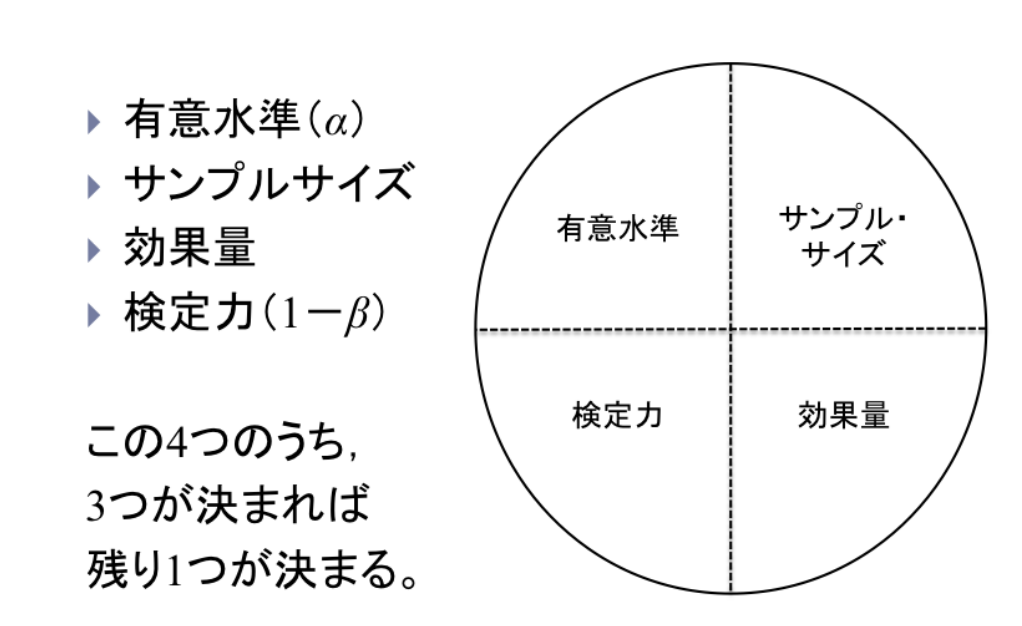
\includegraphics[keepaspectratio,width=0.8\linewidth]{../images/19_NHST2/Slide19_03.png}
    \caption{統計的検定における四つの要素の関係}
    \label{fig::18_04}
\end{figure}

In a hypothesis test, the four essential factors affecting the decision are the significance level, sample size, effect size, and power, among which one element is calculated when three other factors are determined \citep{Mizumoto2010}. Generally, a significance level of 5\% is used, and a power of about 0.8 is recommended. Therefore, the sample size can be determined based on the effect size. If the effect size is small, a large sample size is necessary, and vice versa. However, it is incorrect to assume that "bigger sample size is always better", as a too large sample size may detect even slight differences that are not practically significant.
However, it is often difficult to know the effect size in advance before starting research. Because we don't know how much effect there is, there are many situations where we want to conduct research. However, if there is previous research, it is possible to calculate the sample size and the effect size based on actual data. Therefore, it is possible to calculate the effect size of the study.

Before conducting research, it is called \keytermE{power analysis} to perform pre-calculations. Power analysis is performed in two cases: to design \keytermE{sample size} and to investigate how much \keytermE{effect size} there was after the research. There are statistical packages and R functions available to perform these calculations, so they are actually calculated using them.

\section{Task}
\paragraph{Interpretation of Test Result 0} Assuming a null hypothesis of $\rho=0.0$, a significance test was performed at a 5% level to determine whether the sample correlation coefficient of $r=0.45$ is significant. The alternative hypothesis was accepted. To interpret the results, judge whether the following statement is true or false.
\begin{itemize}
    \item It has been proven that $\rho\neq 0$ in the population.
    \item The probability that $\rho=0$ in the population is less than 5\%.
    \item $\rho$ is a value greater than 0 in the population.
    \item $\rho=0.45$ in the population.
    \item If it is assumed that $\rho=0$ in the population, the probability of obtaining a value of $|r|>0.45$ is less than 5\%.
\end{itemize}


\paragraph{Significance Level and Sample Size} Let's determine whether each of the following statements is true or false.

(Note: This is a literal translation of the Japanese text provided, but it may be more natural to use "Let's" instead of "We" to refer to the reader and translator together.)
\begin{itemize}
    \item 他の条件が一定なら，有意水準が小さくなると有意になりにくくなる。
    \item 他の条件が一定なら，有意水準が小さくなると第二種の誤りを犯す確率が大きくなる。
    \item 他の条件が一定なら，サンプルサイズが大きくなると有意になりやすくなる。
    \item 他の条件が一定なら，サンプルサイズが大きくなると帰無仮説を棄却するときの理論的な統計量の絶対値が大きくなる。
\end{itemize}

\paragraph{Properties and meaning of $p$-values} Let's determine whether the following statements are true or false for each respective sentence.
\begin{itemize}
    \item $p$値が小さいとき，母集団における効果は大きい。
    \item $p$値が小さいとき，帰無仮説が正しい確率は小さい。
    \item $p$値が小さいとき，有意水準は小さい。
    \item $p$値はデータから計算される統計量である。
\end{itemize}

\paragraph{Power Analysis} Please judge whether the following sentences are true or false for each of them. (Note: The TeX code will not be modified.)
\begin{itemize}
    \item If other conditions are constant, the sample size and the testing power increases as well.
    \item Assuming testing power is 0.6, it means there is a 0.4 probability of missing an effect.
    \item To calculate testing power, it is necessary to assume the size of the effect to be detected.
    \item Testing power is the probability that the sample statistic coincides with the unknown population value. 
\end{itemize}


\end{document}
